\chapter{Introduction générale} \label{Chapter1}

\section{Présentation de projet}
Dans le cadre de la formation d’ingénieur de l’École Centrale Casablanca, les élèves de deuxième année doivent réaliser un projet base de données. Celui-ci consiste sur une durée de deux mois avec une fréquence d’une séance par semaine, à conceptualiser et réaliser un système de gestion d’une base de données.
C’est dans cette optique que nous avons eu le plaisir de choisir le thème : système d'inventaire de maison.

Aujourd'hui, les logiciels sont utilisés dans presque tous les domaines de la vie quotidienne. Les téléphones portables, les télévisions, les appareils de chauffage, les voitures et même certains de nos grille-pains sont dotés de logiciels qui les rendent plus faciles à utiliser et améliorent ainsi la vie des personnes qui les utilisent.  Avec l'arrivée de cette nouvelle technologie dans nos voitures et nos téléphones portables, il semble étrange que l'endroit où nous passons le plus de temps soit à la traîne dans cette tendance. Nos maisons sont désormais la prochaine facette de notre vie que nous devrions améliorer.

\begin{figure}[ht]
    \centering
    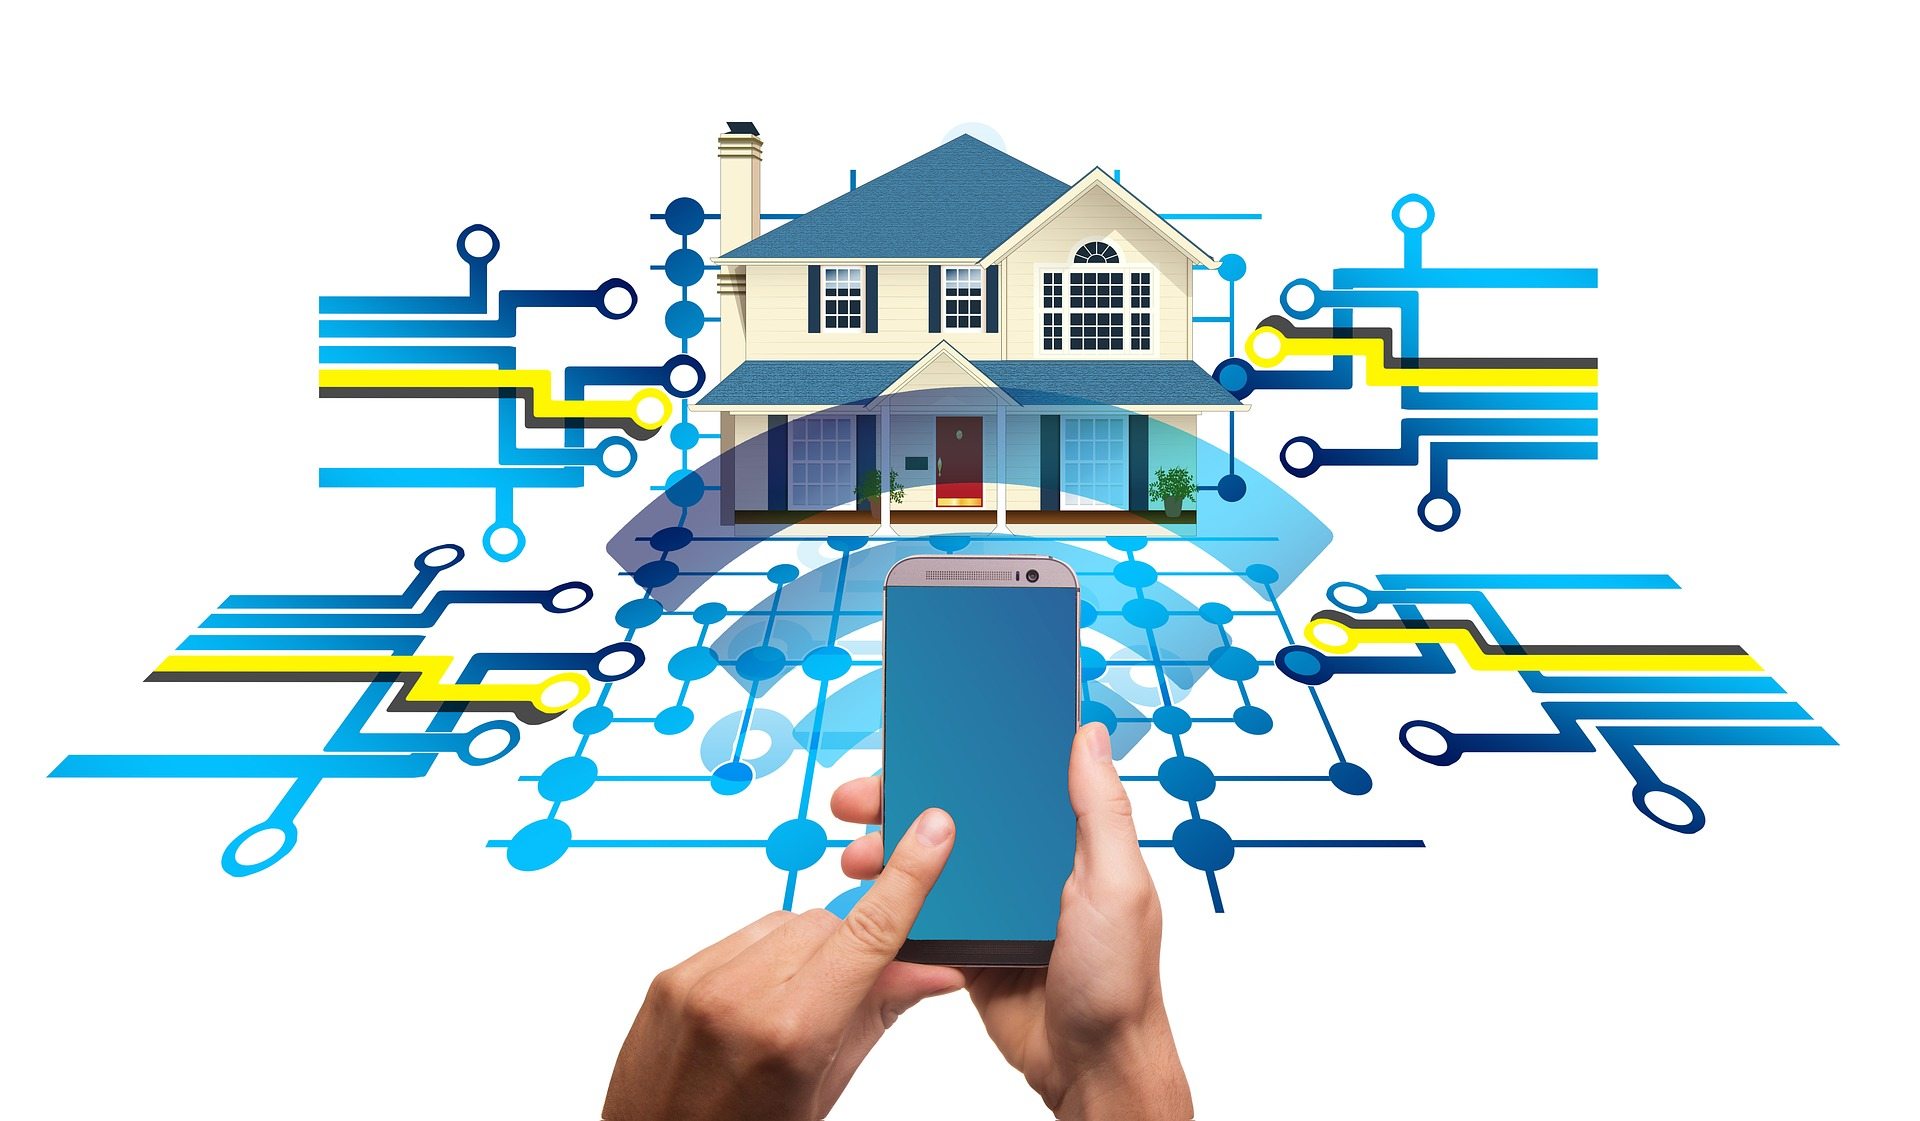
\includegraphics[keepaspectratio=true,scale=0.65]{Figures/smart-home.jpg}
    \caption{Smart Home}
    \label{fig:structure}
\end{figure}

La "Smart Home" est une maison qui utilise les nouvelles technologies pour faciliter la vie de ses occupants. Que vous soyez une personne âgée vivant seule ou un étudiant, chacun peut les utiliser. Avant de pouvoir construire une véritable maison intelligente, nous devons développer les composants qui constitueront la base du système. L'un de ces composants, d'une importance vitale, est un moyen d'organiser et de garder la trace des objets de la maison. Le système d’inventaire de maison est une idée simple qui peut être utilisée comme l'un des composants de la maison intelligente. Imaginez qu'un terrible accident détruise la maison d'un particulier ; il arrive souvent que le compte exact des biens personnels du propriétaire devienne un problème entre lui et la compagnie d'assurance. L'inventaire de la maison résout ce problème en gardant la trace de chaque objet de la maison, ce qui simplifie considérablement le recouvrement des pertes en cas d'accident.

Dans la suite de ce rapport, nous exposerons tous les résultats que nous avons obtenus à l’issu de ce projet.

\section{Plan de travail}
\subsection{Organisation du rapport}
Le rapport est divisé en cinq chapitres principaux décrivant le projet, les processus et les résultats, voir figure \ref{fig:structure}. Le premier chapitre est une introduction au projet. La deuxième partie consiste en une étude préalable sur la méthode que nous allons utiliser, les exigences des utilisateurs ( les exigences sont en gros divisées en deux groupes : les exigences fonctionnelles et les exigences non fonctionnelles ). Le troisième chapitre décrit la première phase du projet qui consiste à réaliser différents diagrammes (dictionnaire des données, MCD, et MLD). Le quatrième chapitre de ce rapport présente le prototype final, une présentation du prototype qui a été développé à partir des résultats identifiés et classés par ordre de priorité.  Pour conclure ce rapport, un dernier chapitre représentant la discussion et la conclusion du rapport est présenté.

\begin{figure}[ht]
    \centering
    
\includegraphics[keepaspectratio=true,scale=0.65]{Figures/structure-rapport.pdf}
    \caption{Structure du rapport}
    \label{fig:structure}
\end{figure}

\subsection{Diagramme de Gantt}
Tout au long de semestre, notre groupe a organisé des réunions, pendant lesquelles plusieurs aspects de la solution sont discutés. Les différentes composantes de notre produit final ont été choisi par le groupe, après plusieurs recherches. Le tableau et le diagramme Gant ci-dessous montrent les étapes de réalisation du prototype.

\begin{figure}[ht]
    \centering
    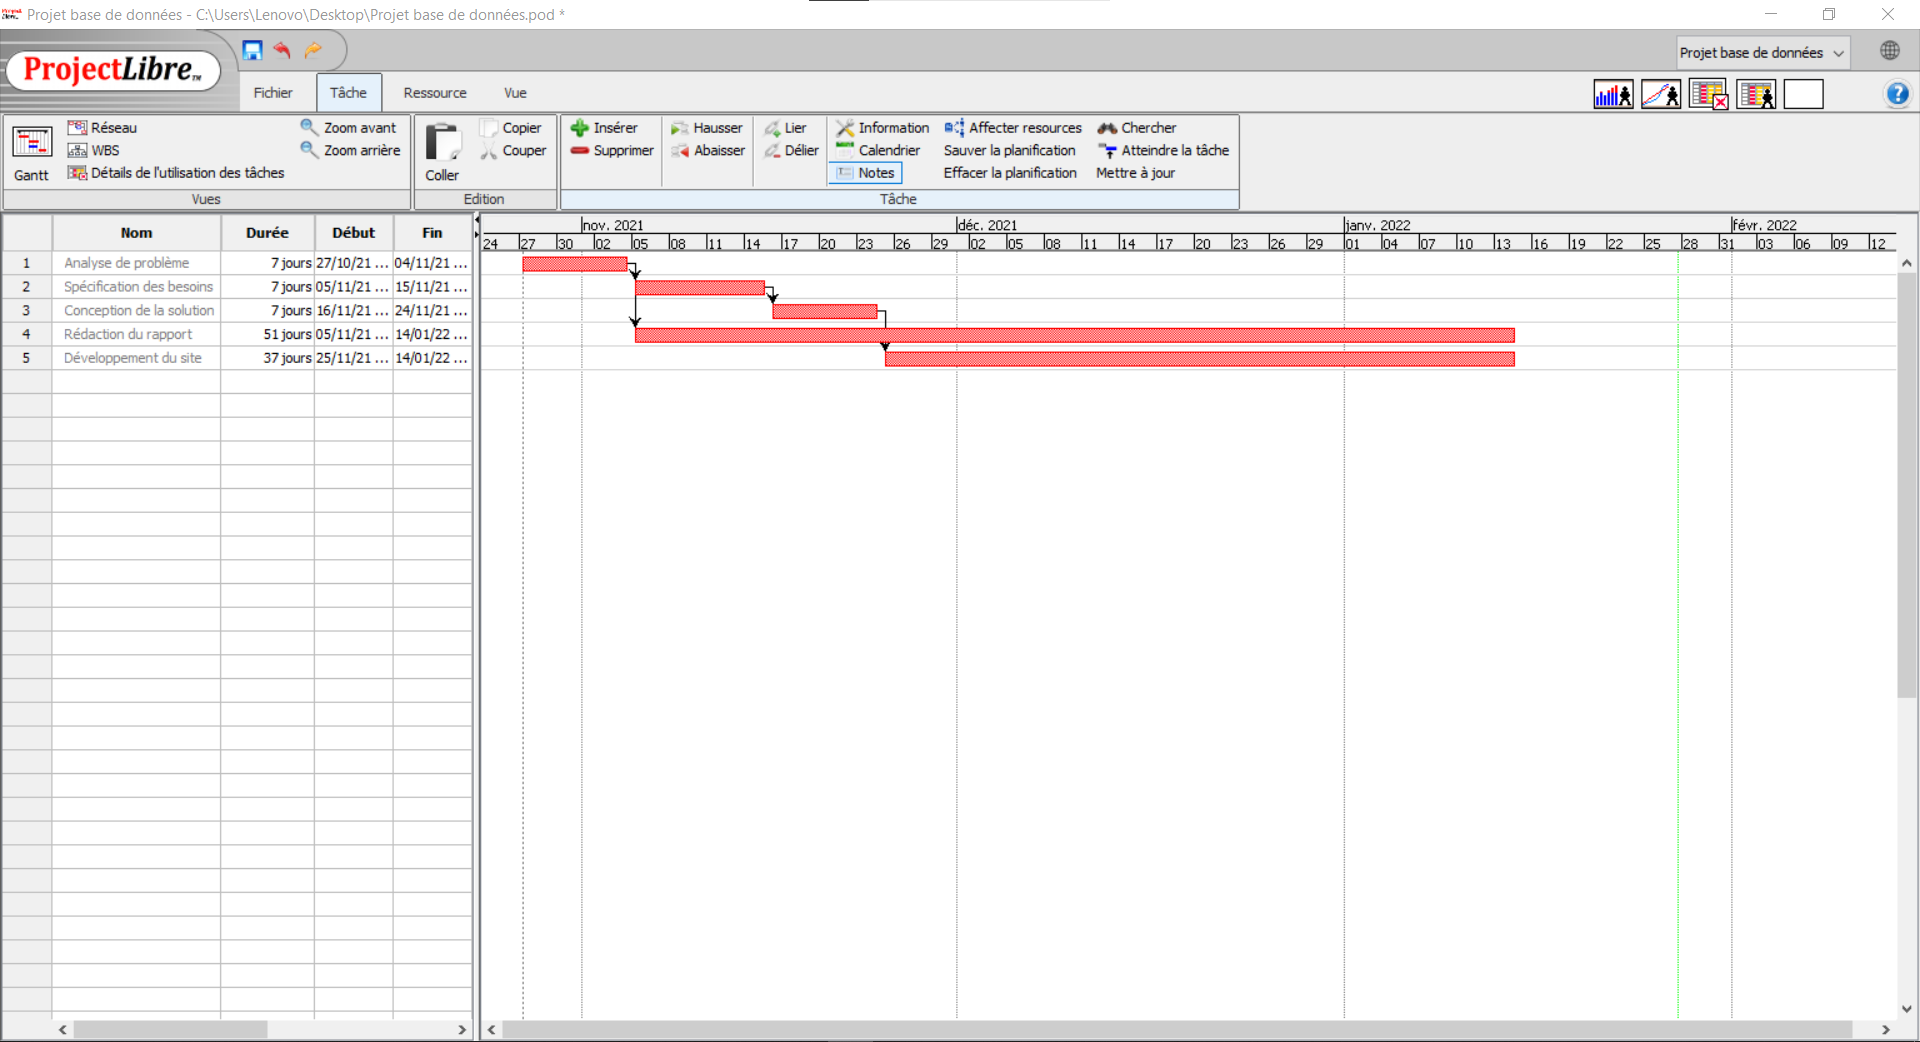
\includegraphics[keepaspectratio=true,scale=.6, angle = -90]{Figures/gantt.png}
    \caption{Diagramme de Gantt}
    \label{fig:structure}
\end{figure}
